\documentclass[12pt]{article}

\usepackage{sbc-template}

\usepackage{graphicx,url}
\usepackage{csvsimple}
\usepackage{subfigure}

\usepackage{amssymb}% http://ctan.org/pkg/amssymb
\usepackage{pifont}% http://ctan.org/pkg/pifont
\newcommand{\cmark}{\ding{51}}%
\newcommand{\xmark}{\ding{55}}%

\usepackage{multirow}
\usepackage[brazil]{babel}    
\usepackage[utf8]{inputenc}
 
\sloppy

\title{Extensão de um elemento de artigo}

\author{Gustavo Ciotto Pinton\inst{1} }


\address{Instituto de Computação -- Universidade Estadual de Campinas
(UNICAMP)\\
  Av. Albert Einstein, 1251, Cidade Universitária, Campinas/SP \\
  Brasil, CEP 13083-852, Fone: [19] 3521-5838
  \email{ra117136@unicamp.br}
}

\begin{document} 

\maketitle

\begin{abstract}
This report extends the results obtained in report 3 and appends two new curves:
one representing 4KB memory pages and the other, 4MB memory pages. In this case,
according to the orientation given during class, all results were
calculated (or recalculated) for the \texttt{SPEC CPU2006} benchmarks containing
100 million instructions in the warm up region and 30 million instructions in
the detailed region. As in the previous case, we used micro-archicteture
simulator sniper and its internal structure was modified in order to reflect the
desired configuration. We discussed the effects of different page sizes on
the measured IPC and considered a page table with a three-level hierarchy. 
\end{abstract}
     
\begin{resumo} 
Este relatório estende os resultados obtidos no relatório 3 e acrescenta duas
novas curvas: uma para páginas de memória com 4KB e a outra, para 4MB. Neste
caso, de acordo com a orientação do professor durante as aulas, todos os
resultados foram calculados (ou recalculados) para os \textit{pinballs} com 100
milhões de instruções na região de warm-up e 30 milhões na região detalhada dos
benchmarks do \texttt{SPEC CPU2006}. Assim como no caso anterior, o simulador de
micro-arquiteturas sniper foi utilizado e sua estrutura interna foi modificada a
fim de refletir os estados desejados. Nós discutimos os efeitos da alteração do
tamanho das páginas no IPC medidos e consideramos uma hierarquia de três níveis
para a tabela de páginas. 
\end{resumo}


\section{Introdução}

O artigo escolhido para os projetos 3 e 4 foi \textit{Accelerating Decoupled
Look-ahead via Weak Dependence Removal: A Metaheuristic Approach} \cite{artigo}.
Neste artigo, em poucas palavras, os autores propuseram uma maneira a partir de
algoritmos genéticos de melhorar o desempenho da \textit{thread} auxiliar
(chamada também de \textit{look-ahed thread}) que, segundo seus experimentos,
torna-se o limitante da performance dos programas \textit{single-threaded} que
são executados neste tipo de arquitetura. Um resumo completo do artigo e do
relatório 3 pode ser encontrado em \cite{relatorio3}.

No projeto 3, implementamos as curvas \textit{ideal} e \textit{single-thread} da
figura \ref{fig:artigo} (figura 3 da página 3 de \cite{artigo}). Propõem-se,
neste relatório, adicionar dois novos resultados a este gráfico, referentes a
páginas de memória de 4KB e de 4MB.
Diferentemente do projeto 2 \cite{relatorio2}, em que o objetivo foi avaliar o
número de acessos adicionais à  memória devido a \textit{misses} nas TLBs, o
intuito deste relatório é avaliar os efeitos da mudança do tamanho das páginas
no IPC. Assim como em \cite{relatorio3}, utilizamos o \textit{sniper} como
simulador e modificamos algumas de suas classes para permitir a especificação do
tamanho de tais páginas. Essas modificações serão detalhadas nas próximas
seções.

\begin{figure}[h!]
  \centering
  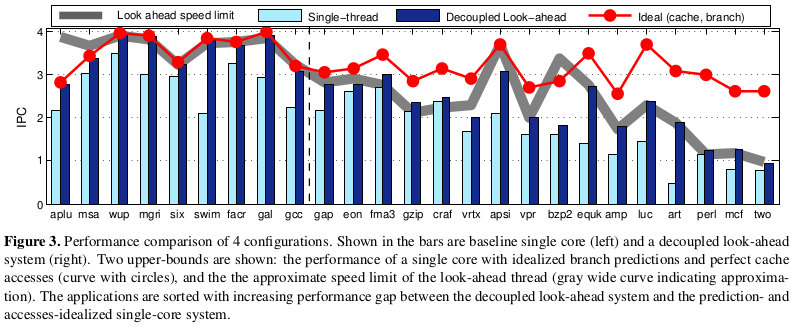
\includegraphics[width=\textwidth]{img/fig3}%
  \label{fig:artigo}%
  \caption{Figura escolhida para reprodução em \cite{relatorio3} com legenda
  original. Extraída de \cite{artigo}.}
\end{figure}

No projeto 2 \cite{relatorio2}, concluimos que o número de acessos a memória era
superior para páginas de 4KB. Adicionalmente, para alguns \textit{benchmarks}
testados nesta ocasião, o número de acessos ocasionadas por \textit{misses} na TLB
correspondia a uma fração importante do número total de acessos. Entretanto,
discutimos também que, apesar disso, o desempenho no caso de 4MB não era
necessariamente melhor que para 4KB, visto que páginas de 4MB
introduziriam uma forte fragmentação da memória já que até processos
utilizando menos de 4MB teríam uma página completa alocada na memória. 

A configuração do ambiente utilizado neste relatório seguiu aquela especificada
em \cite{relatorio3}. Entretanto, ao invés de usar \textit{pinballs} de
\textit{benchmarks} do \texttt{SPEC CPU2006} com 1 bilhão de instruções na
região detalhada e sem \textit{warm up}, utilizamos aqueles com 100 milhões de
intruções de aquecimento e 30 milhões para a região de interesse. Estes últimos
oferecem resultados mais próximos dos originais, uma vez que eliminam os efeitos 
dos \textit{misses} e \textit{mispredictions} iniciais. Além disso, recalculamos
os resultados obtidos em \cite{relatorio3} para tais \textit{pinballs}.

Consideramos para este relatório que a tabela de páginas contém 3 níveis de
hierarquia. Dessa forma, a fim de simular esse comportamento, foi necessário
o estudo do código do \textit{sniper} e a identificação dos parâmetros que
pudessem adicionar a latência de 3 acessos adicionais a memória em caso de um
eventual \textit{miss} nas TLBs de instruções e dados. As modificações
realizadas podem ser encontradas na seção \textbf{Implementação}, a seguir.

\section {Implementação}

Nesta seção, serão discutidos detalhes da implementação, tais como modificações
em classes do \textit{sniper} e na sua configuração. Destaca-se, conforme já
mencionado na seção anterior, que estendemos a configuração apresentada no
relatório do projeto 3 \cite{relatorio3} para incluir páginas de memória de
diferentes tamanhos.

\subsection{Modificação do \textit{sniper}}

As TLBs são implementados pelo simulador \textit{sniper} através da classe
\texttt{TLB}, declarada no arquivo \texttt{tlb.h} e definida em \texttt{tlb.cc}.
Originalmente, essa classe possui três contantes, sendo elas
\texttt{SIM\_PAGE\_SHIFT}, \texttt{SIM\_PAGE\_SIZE} e \texttt{SIM\_PAGE\_MASK},
representando, respectivamente, o deslocamento em bits que deve ser efetuado no
endereço a ser traduzido, o tamanho de uma paǵina de memória e a máscara a ser
utilizada. É importante observar que \texttt{SIM\_PAGE\_SIZE} e
\texttt{SIM\_PAGE\_MASK} são definidos por um único parâmetro, sendo ele
\texttt{SIM\_PAGES\_SHIFT}. Dessa maneira, qualquer modificação neste último,
altera todo o comportamento na classe. Por padrão, o \textit{sniper} define o
valor de \texttt{SIM\_PAGE\_SHIFT} igual a 12, utilizando
assim páginas de 4KB (4KB = \(2^{12}\)). Para o uso de páginas de 4MB, por sua
vez,  \texttt{SIM\_PAGE\_SHIFT} deve valer 22 (4MB = \(2^{22}\)).

Modificamos, portanto, o \textit{sniper} e transformamos as constantes do
parágrafo em variáveis. Adicionamos ao construtor da classe um novo parâmetro,
chamado de \path{page_size_bits}, que determina o valor de
\path{SIM_PAGE_SHIFT} e, em consequência, de \path{SIM_PAGE_SIZE} e
\path{SIM_PAGE_MASK}. A determinação deste novo parâmetro é realizada a partir
da opção \path{page_size_bits}, lida dos arquivos de extensão \texttt{.cfg}.

Alteramos o construtor da classe \texttt{MemoryManager}, implementado
no arquivo \path{memory_manager.cc}, para a leitura desta nova opção e
recompilamos o \textit{sniper}. O arquivo de configuração \texttt{base.cfg} que
serve como base para todas as configurações define a opção \path{page_size_bits}
como 12. Assim, configurações criadas anteriormente às modificações desta
seção continuarão a utilizar as páginas padrões de 4KB.

Enfim, atribuímos à propriedade \texttt{penalty} de \path{perf_model/tlb} o
valor de 600 (\(3\times 200\)), especificando assim a penalidade de três acessos
adicionais à memória em caso de um \textit{miss} em qualquer das TLBs.

\subsection{Correção na propriedade \textit{latency} da memória}

No relatório 3 \cite{relatorio3}, citamos que o a latência de memória
correspondia a 200 ciclos. Nesta ocasião, atribuímos à propriedade
\path{latency} de \path{perf_model/dram} o valor de 200. Entretanto, o
\textit{sniper} interpreta este valor como \textit{nanossegundos} e não ciclos.
Dessa forma, a latência especificada corresponde a um valor muito superior
daquela desejada, isto é, 87ns (para a frequência de 2.3GHz, 200 ciclos
equivalem a \(200*\frac{1}{2.3\times 10^9} \approx 87ns\)). Portanto, os valores
de IPC encontrados em \cite{relatorio3} foram um pouco inferiores aos desejados.
Entretanto, como este parâmetro foi usado para todos os \textit{benchmarks}, a
forma das curvas encontrada deve se manter igual àquela encontrada neste
relatóriom na seção \textbf{Resultados}.

\subsection{Estrutura das \textit{caches}}

Escolhemos utilizar a estrutura de caches implementado na configuração da
micro-arquitetura \textit{Nehalem}, presente por padrão no \textit{sniper}. Dois
níveis de \textit{cache} estão presentes, sendo que o segundo é compartilhado
entre as TLBs de dados e instruções. 

A TLB de instruções possui 128 entradas e é \textit{4-way associative}. A de
dados, por sua vez, possui a metade de entradas, isto é, 64, e também é
\textit{4-way associative}. Por fim, a TLB compartilhada possui 512 entradas e,
como as duas anteriores, é \textit{4-way associative}. 

\section{Resultados}

\section{Conclusões}


\bibliographystyle{sbc}
\bibliography{sbc-template}

\end{document}
